\documentclass[fleqn]{article}
\author{Authors from Deltares and USGS}

\usepackage{amsmath}
\usepackage{xcolor}
\usepackage{graphicx}
\graphicspath{{./figures/}}


\begin{document}

\title{Surface Water Flow in MODFLOW 6}
\maketitle

\tableofcontents

\section{Theoretical Development}
In this section ...

\subsection{Conservation of Mass}
Partial differential equation on conservation of mass:

\subsection{Manning's Equation}
Manning's equation is given as

\begin{equation}
  Q = \frac{1}{n} A R^{2 \over 3} \sqrt{S_f}
\end{equation}

\subsection{Storage Term}
The change in mass of water 

\subsection{Channel Cross Sections}

\section{Numerical Solution}

\subsection{Newton-Raphson Method}

Flow throughout the connected channel network is based on a Newton-Raphson formulation, in which the following equation is formulated and solved simultaneously for each reach \textcolor{red}{change n and m to i and j?}

\begin{equation}
\label{eqn:nr-cvfd}
\begin{split}
\left ( \sum\limits_{m \in \eta_{n}} \frac{\partial Q_{n,m}}{\partial h_n} + \frac{\partial Q_{n,s}}{\partial h_n} - \frac{\partial Q_{STO}}{\partial h_n} \right ) h^k_n + 
\sum\limits_{m \in \eta_{n}} \frac{\partial Q_{n,m}}{\partial h_m} h^k_{m} = \\
- \left ( \sum\limits_{m \in \eta_{n}} Q_{n,m} + Q_{n,s} - Q_{STO} \right ) + \\
\left ( \sum\limits_{m \in \eta_{n}} \frac{\partial Q_{n,m}}{\partial h_n} + \frac{\partial Q_{n,s}}{\partial h_n} - \frac{\partial Q_{STO}}{\partial h_n} \right ) h^{k-1}_n + \sum\limits_{m \in \eta_{n}} \frac{\partial Q_{n,m}}{\partial h_m} h^{k-1}_{m}.
\end{split}
\end{equation}

\subsection{Linear Network}

% This figure below is for the case where roughness varies for each line segment in the cross section 
\begin{figure}
	\centering
	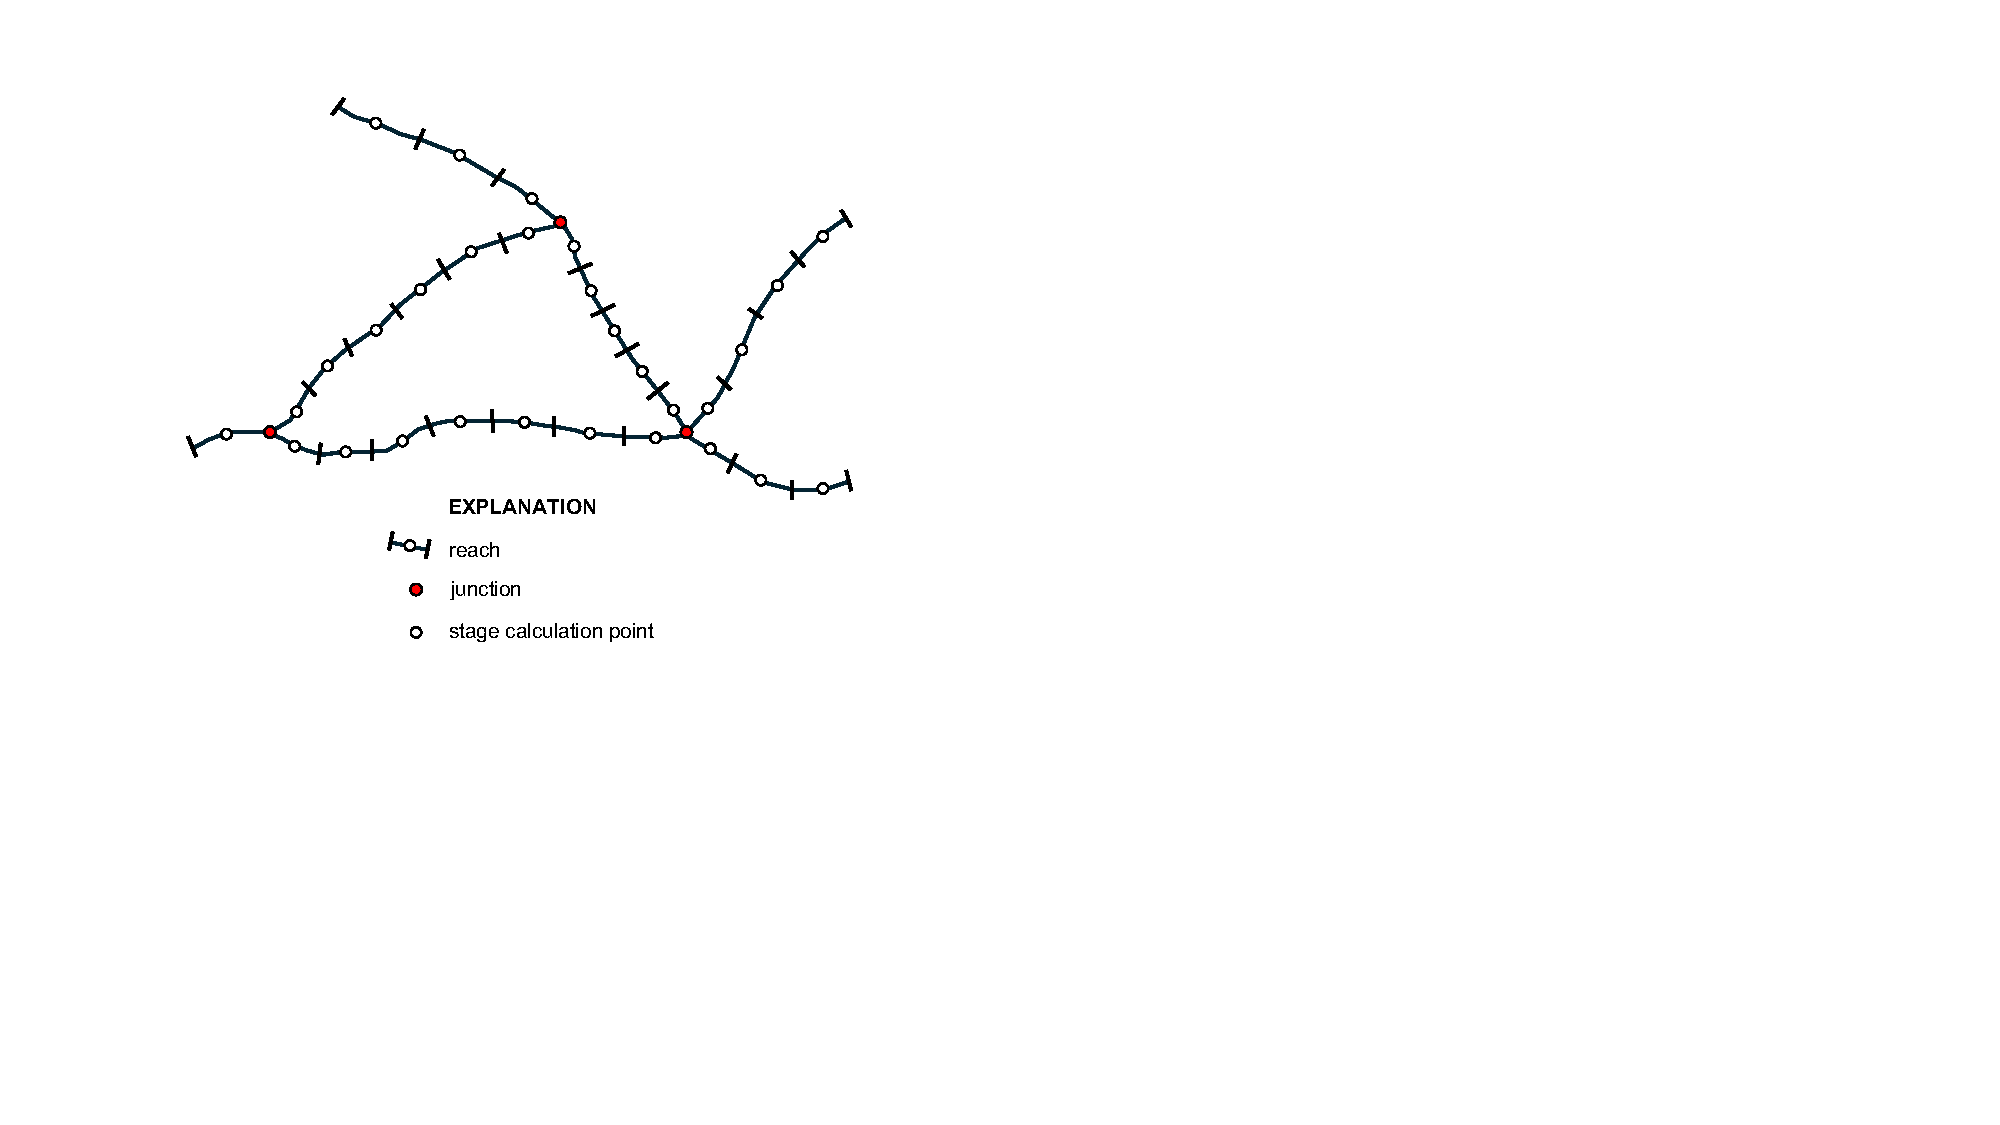
\includegraphics[scale=0.9]{figures/channel_network.pdf}
	\caption[Schematic showing a channel network.]{Schematic showing a channel network.  The channel network is discretized by the user into computational elements called reaches.  Stage is calculated within the reach at stage calculation points.}
	\label{fig:channel_network}
\end{figure}


\subsection{Discretized Flow Expression}

Manning's equation is written as

\begin{equation}
  Q = \frac{1}{n} A R^{2 \over 3} \sqrt{S_f}
\end{equation}

\noindent where $R$ is the hydraulic radius equal to $A / P$.  For the numerical implementation in MODFLOW we express Manning's equation as a product of a conductance term and the product of the head difference between reach $n$ and $m$

\begin{equation}
  Q_{nm} = C_{nm} \left ( h_m - h_n \right )
\end{equation}

\noindent The average conductance between the two cells $C_{nm}$ is calculated using the following harmonic mean, which consists the half-cell conductance in reach $n$ and the half-cell conductance in reach $m$

\begin{equation}
  C_{nm} = \frac{C_n  C_m}{C_n + C_m}
\end{equation}

The half-cell conductance for a reach, $n$, is calculated as

\begin{equation}
  C_n = \frac{B_n}{ L_{nm} \sqrt{ \frac{ | \left ( h_m - h_n \right ) | } {L_{nm} + L_{mn}}} }
\end{equation}

\noindent where $B_n$ is the conveyance for reach $n$.  Conveyance is calculated in several different ways depending on how the cross section is defined.  For the cross sections shown in figure \ref{fig:cxs} a single Manning's roughness coefficient is assigned for the section.  If a single Manning's roughness coefficient is used, then the conveyance is calculated as

\begin{equation}
  B = \frac{A R^{2 \over 3}}{n}
\end{equation}

% This figure below is for the case where roughness is the same for every line segment in the cross section 
\begin{figure}
	\centering
	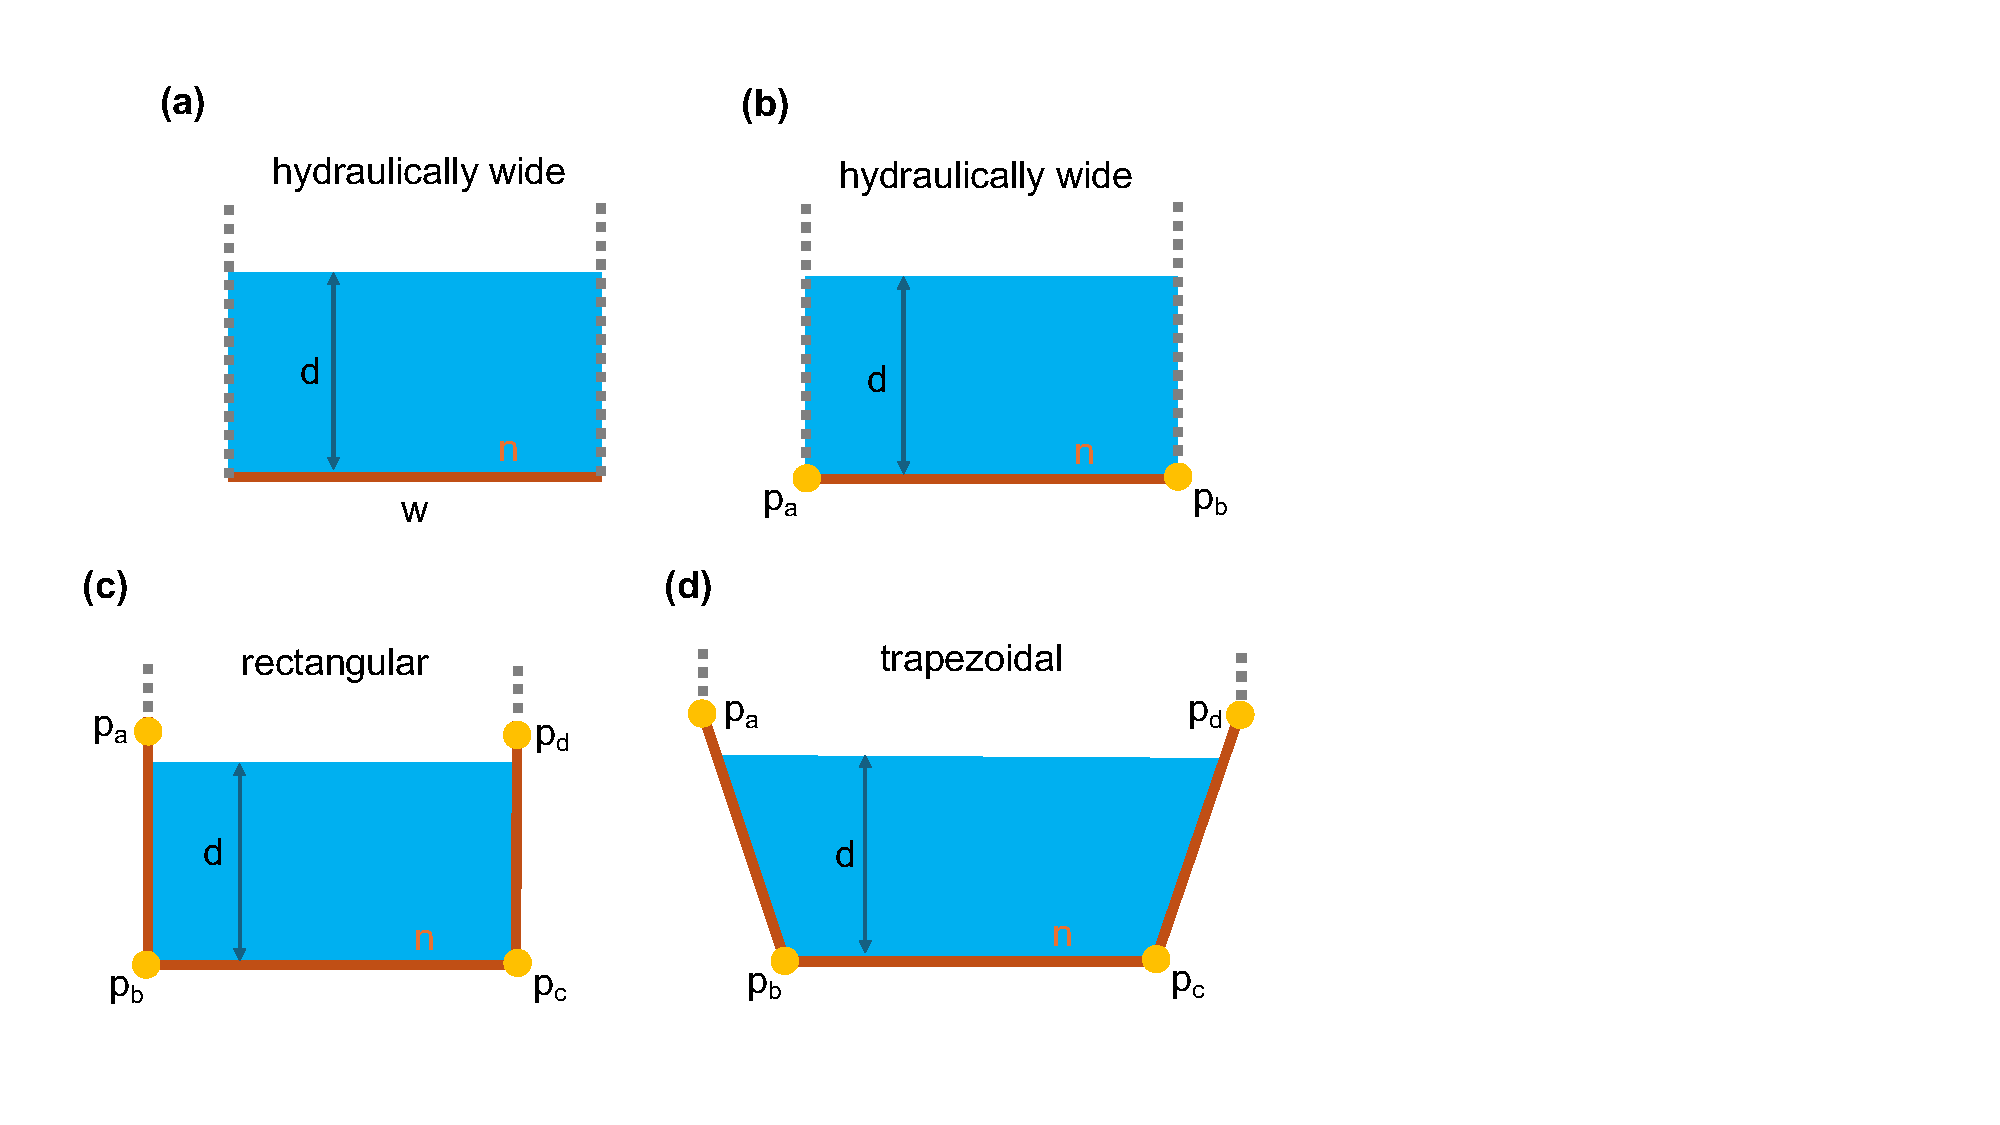
\includegraphics[scale=0.5]{figures/cxs.pdf}
	\caption[Schematic showing different types of channel cross sections with constant roughness.]{Schematic showing different types of cross sections with a single Manning's roughness coefficient $n$: (a) hydraulically wide cross section defined using the width input parameter; (b) hydraulically wide cross section defined using two points; (c) a rectangular cross section defined using four points, and (d) a trapezoidal cross section defined using four points.  For the hydraulically wide rectangular cross sections in (a) and (b) the model does not include any channel resistance for the vertical wetted sections corresponding to the dashed lines.  For cross sections shown in (c) and (d), if the water surface rises above the channel points, no channel resistance is included for sections above the uppermost points}
	\label{fig:cxs}
\end{figure}

If a cross section does not have a constant Manning's roughness coefficient for all line segments that define the channel, then a composite conveyance is calculated by summing the individual conveyance parts for the channel as

\begin{equation}
  B = \sum_{i=1}^{NLS} \frac{A_i \left ( \frac {A_i}{P_i}\right )^{2 \over 3}}{n_i}
\end{equation}


% This figure below is for the case where roughness varies for each line segment in the cross section 
\begin{figure}
	\centering
	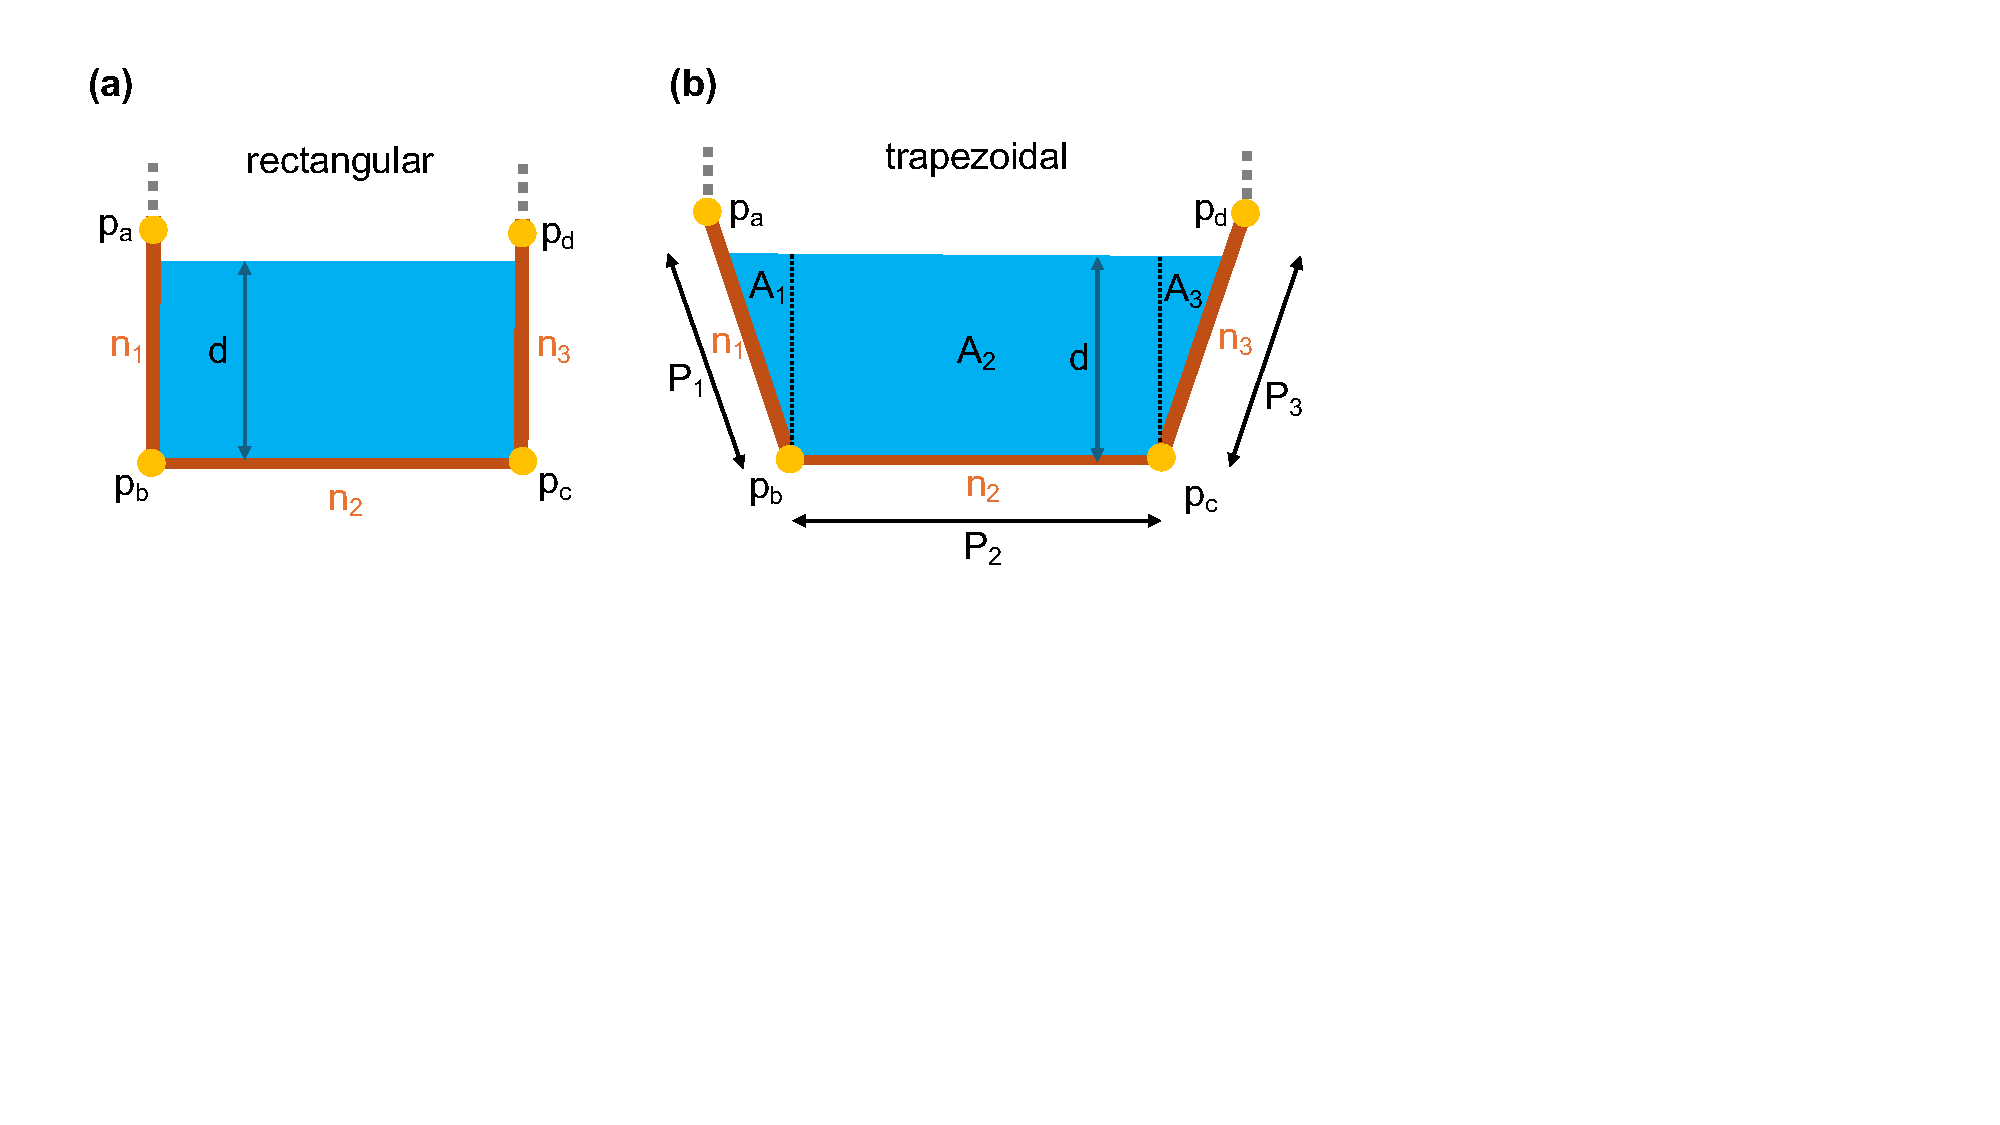
\includegraphics[scale=0.5]{figures/cxs_rough.pdf}
	\caption[Schematic showing different types of channel cross sections with variable roughness.]{Schematic showing different types of cross sections with variable Manning's roughness coefficient: (a) a rectangular cross section defined using four points, and (b) a trapezoidal cross section defined using four points.  The Manning's roughness coefficient is varies by line segment.  If the water surface rises above the channel points, no channel resistance is included for sections above the uppermost points}
	\label{fig:cxs_rough}
\end{figure}


\subsection{Temporal Discretization}
Adaptive time stepping

\subsection{Sources and Sinks}

\subsection{Initial and Boundary Conditions}

A zero-depth-gradient (ZDG) boundary condition can be assigned to any reach to allow from the channel.  Flow out of the channel is calculated as

\begin{equation}
  Q = \frac{1}{n}A R^{2/3} \sqrt{S_0}
\end{equation}


\section{Integration into MODFLOW 6}

\section{Model Verification}

\subsection{Analytical Results}

\subsection{Example Problems}

\end{document}